\documentclass[8pt]{beamer}

\newif\ifplacelogo % create a new conditional
\placelogotrue % set it to true

\usetheme{Warsaw}
\usecolortheme{rose}
\usepackage{multicol}
\usepackage{epstopdf}
\usepackage[italic]{hepnames}
\usepackage{tikz}
\usepackage{listings}
\usepackage{times}
\usepackage{amsmath}
\usepackage{verbatim}
\usepackage{hyperref}
\usepackage{bbding}
\lstset{breakatwhitespace,
language=C++,
columns=fullflexible,
keepspaces,
breaklines,
tabsize=3, 
showstringspaces=false,
extendedchars=true}

% TikZ includes!!!
\usepackage{tikz}
\usetikzlibrary{backgrounds}
\usetikzlibrary{calc}
\tikzstyle{every picture}+=[remember picture]
\input{/home/oviazlo/Desktop/beamerPresentations/myReports/latexHelpScripts/tikzGrid.tex}


\begin{document}

% custom colors
\definecolor{olive}{rgb}{0.3, 0.4, .1}
\definecolor{fore}{RGB}{249,242,215}
\definecolor{back}{RGB}{51,51,51}
\definecolor{title}{RGB}{255,0,90}
\definecolor{dgreen}{rgb}{0.,0.6,0.}
\definecolor{gold}{rgb}{1.,0.84,0.}
\definecolor{JungleGreen}{cmyk}{0.99,0,0.52,0}
\definecolor{BlueGreen}{cmyk}{0.85,0,0.33,0}
\definecolor{RawSienna}{cmyk}{0,0.72,1,0.45}
\definecolor{Magenta}{cmyk}{0,1,0,0}

\definecolor{PixelColor}{RGB}{207,232,139}
\definecolor{SCTColor}{RGB}{167,166,255}
\definecolor{TRTColor}{RGB}{250,224,140}
\definecolor{grayColor}{RGB}{153,153,153}

\newcommand{\yRefPosOne}{0.0}
\newcommand{\xRefPosOne}{0.0}
\newcommand{\yRefPosTwo}{0.0}
\newcommand{\xRefPosTwo}{0.0}
\newcommand{\yRefIncrementOne}{0.0}
\newcommand{\xRefIncrementOne}{0.0}
\newcommand{\yRefIncrementTwo}{0.0}
\newcommand{\xRefIncrementTwo}{0.0}

\graphicspath{ {/home/oviazlo/Desktop/beamerPresentations/FCCee/pictures/plots_CALICE_workshop/} }


\DeclareGraphicsExtensions{.eps, .pdf, .png}

\newcommand{\myBox}[2][pink] {
    \noindent\colorbox{#1}{
	\textbf{#2}
    }\par
}

% For nice block (provided by Oleh)
\tikzstyle{myBox} = [draw=red, fill=blue!1, very thick,
    rectangle, rounded corners, inner sep=5pt, inner ysep=9pt]
    
\tikzstyle{PixelBox} = [draw=PixelColor, fill=blue!1, very thick,
    rectangle, rounded corners, inner sep=5pt, inner ysep=9pt]
\tikzstyle{SCTBox} = [draw=SCTColor, fill=blue!1, very thick,
    rectangle, rounded corners, inner sep=5pt, inner ysep=9pt]
\tikzstyle{TRTBox} = [draw=TRTColor, fill=blue!1, very thick,
    rectangle, rounded corners, inner sep=5pt, inner ysep=9pt]

% poster advertisement
\newcommand{\myCenterBox}[2][pink] {
   {\centering
    \noindent\colorbox{#1}{
	\textbf{#2}
    }\par
  }
}

\newcommand{\mySmallCenterBox}[2][pink] {
   {\centering
    \noindent\colorbox{#1}{
	\textbf{{\small #2}}
    }\par
  }
}

\newcommand{\myVerySmallCenterBox}[2][pink] {
   {\centering
    \noindent\colorbox{#1}{
	\textbf{{\scriptsize #2}}
    }\par
  }
}

\newcommand{\backupbegin}{
   \newcounter{finalframe}
   \setcounter{finalframe}{\value{framenumber}}
}
\newcommand{\backupend}{
   \setcounter{framenumber}{\value{finalframe}}
}

\newcommand{\myNode}{\tikz[baseline,inner sep=1pt] \node[anchor=base]}

\tikzstyle{fancytitle} =[fill=white!15, text=black]

\definecolor{light-gray}{gray}{0.95}
% poster advertisement


\title[ Pandora PFA FCC-ee \hspace{19.5em}\insertframenumber/
\inserttotalframenumber]{FCC-ee calorimetery }


	\author[Oleksandr Viazlo]{Oleksandr Viazlo\\ 
% 	{\small ???}
	}
	\institute{\small CERN\\} 
	
       
	\date{21 March 2018}

% 	\logo{ \ifplacelogo \includegraphics[height=1.8cm]{./ID_week2/lund_uni-logo_s.pdf} \hspace{0.4cm} \fi}

	
   	\frame{\titlepage}

   	

\placelogofalse


%*****************************************************************************
\begin{frame}{}
    \begin{tikzpicture}[overlay]
    \node[right] (textNode) at (3.1,0) {
      {\large \bf Single particle efficiency}
    };
    \end{tikzpicture}
\end{frame}
%*****************************************************************************
%*****************************************************************************
\begin{frame}{\large \large Single particle efficiency definition}
 
\renewcommand{\yRefPosOne}{0.4}
\renewcommand{\xRefPosOne}{2.5}
\renewcommand{\xRefIncrementOne}{5.5}
\begin{tikzpicture}[overlay]


\node  at (\xRefPosOne+2.5,\yRefPosOne) (box){%
  \begin{minipage}{\textwidth}
    \begin{itemize}
      \item Single particle performance is studied for $\mu$-, $\pi$-, $e$- and $\gamma$  \\ \vspace{0.2cm}
      \item Simulate single particles with isotrop $cos(\theta)$ distribution and fixed energy: \\5, 10, 20 ,50 and 100 GeV \\ \vspace{0.2cm} 
%       \item Reconstucted PFO is efficient when: \\ \vspace{0.1cm}
     \item PID efficiency definition: \\ \vspace{0.1cm}
      \begin{itemize}
       \item reconstructed PFO and true (MC) particle have to be of the same type
       \item angular matching: $\Delta\theta <$ 0.01rad and $\Delta\phi <$ 0.02rad
       \item energy matching:\\
       - charged particles: $|p_T^{truth} - p_T^{PFO}| < 5\%$ $p_T^{truth} $ \\
       - photons: $\Delta$$E < 5\times\sigma$(ECal) $\approx 0.75\times \sqrt{E}$
       
      \end{itemize}

    \end{itemize}
  \end{minipage}
};

\node at (\xRefPosOne+2.5,\yRefPosOne-4) (box){%
  \begin{minipage}{1.05\textwidth}
    \begin{itemize}
      \item reconstructed PFO types: $\mu\pm$, $e\pm$, $\gamma$, charged hadrons ($\pi\pm$) and neutral hadrons (n)
    \end{itemize}
  \end{minipage}
};

\end{tikzpicture}

  
\end{frame}
%*****************************************************************************
%*****************************************************************************
\begin{frame}{\large \large Single muon efficiency}

\renewcommand{\yRefPosOne}{-0.5}
\renewcommand{\xRefPosOne}{5.5}
\renewcommand{\xRefIncrementOne}{5.5}
\begin{tikzpicture}[overlay]

 \node[inner sep=0pt] (tmp) at (\xRefPosOne-3,\yRefPosOne+1.2)
    {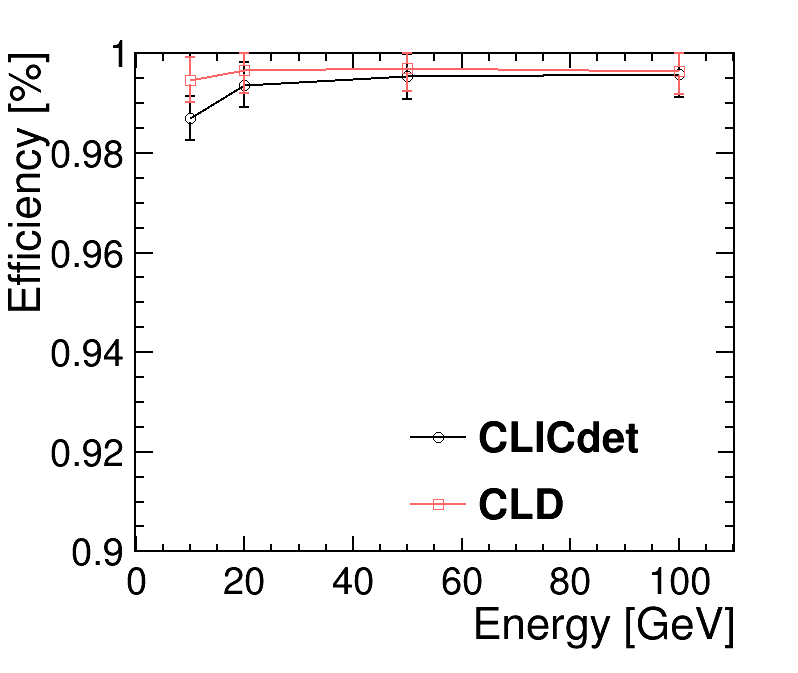
\includegraphics[width=6.2cm]{partEff/experimental_v1/calice_CLIC_vs_FCCee_effVsEnergy_muons.pdf}};
    
 \node[inner sep=0pt] (tmp) at (\xRefPosOne+3,\yRefPosOne+1.25)
    {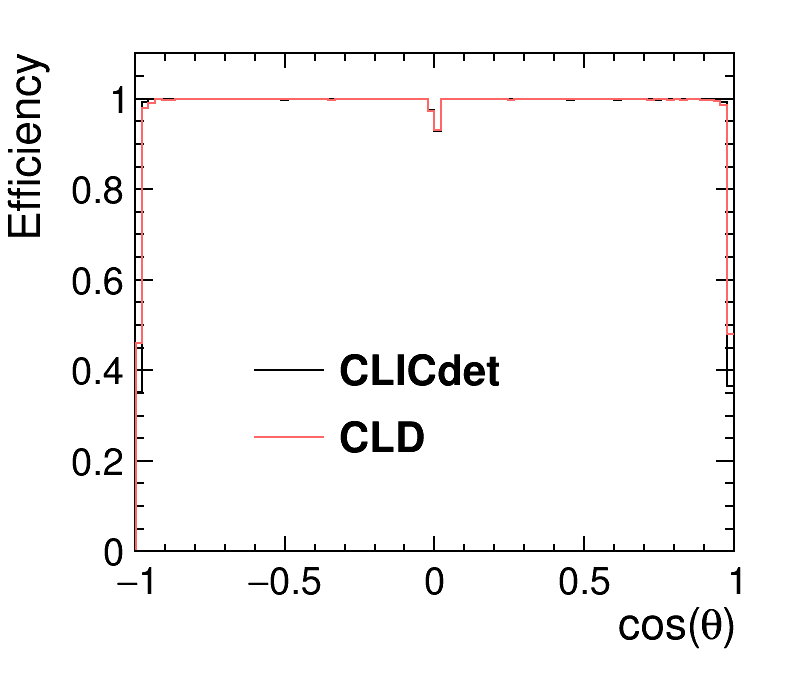
\includegraphics[width=6.2cm]{partEff/experimental_v1/calice_CLIC_vs_FCCee_effVsTheta_muons_E50.pdf}};

\node  at (\xRefPosOne+4.5,\yRefPosOne+3.6) (box){%
\myCenterBox{\small 50 GeV muons}
}; 

 \node[inner sep=0pt] (tmp) at (\xRefPosOne-3.9,\yRefPosOne+3.6)
    {\tiny WORK IN PROGRESS};
 \node[inner sep=0pt] (tmp) at (\xRefPosOne+2.1,\yRefPosOne+3.6)
    {\tiny WORK IN PROGRESS};

\node  at (\xRefPosOne,\yRefPosOne-2.8) (box){%
\begin{minipage}{\textwidth}
  \begin{itemize}
   \item Type, angular and energy matching with the true muon
   \item Muon efficiency is 99$\%$ or larger for all energies both for CLICdet and CLD
   \item Small inefficiency at cos$(\theta) = 0$ due to reconstruction algorithm $\to$ work ongoing
  \end{itemize}
\end{minipage}
};


% % HELPER draw advanced helping grid with axises:
% \draw(-0.5,-4) to[grid with coordinates] (11.5,4);
\end{tikzpicture}
 
\end{frame}
%*****************************************************************************
%*****************************************************************************
\begin{frame}{\large \large Single pion efficiency}

\renewcommand{\yRefPosOne}{-0.5}
\renewcommand{\xRefPosOne}{5.5}
\renewcommand{\xRefIncrementOne}{5.5}
\begin{tikzpicture}[overlay]

 \node[inner sep=0pt] (tmp) at (\xRefPosOne-3,\yRefPosOne+1.2)
    {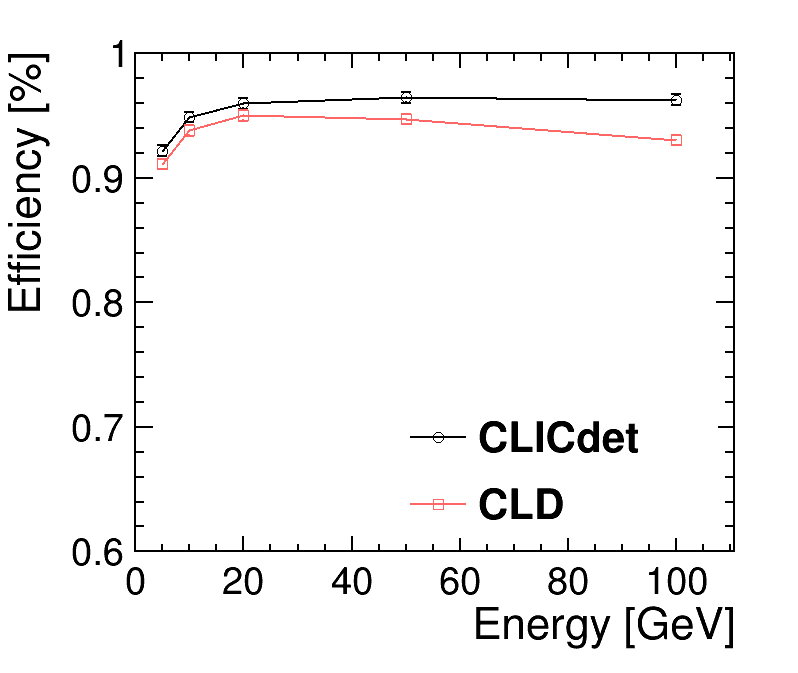
\includegraphics[width=6.2cm]{partEff/experimental_v1/calice_CLIC_vs_FCCee_effVsEnergy_pions.pdf}};
    
 \node[inner sep=0pt] (tmp) at (\xRefPosOne+3,\yRefPosOne+1.25)
    {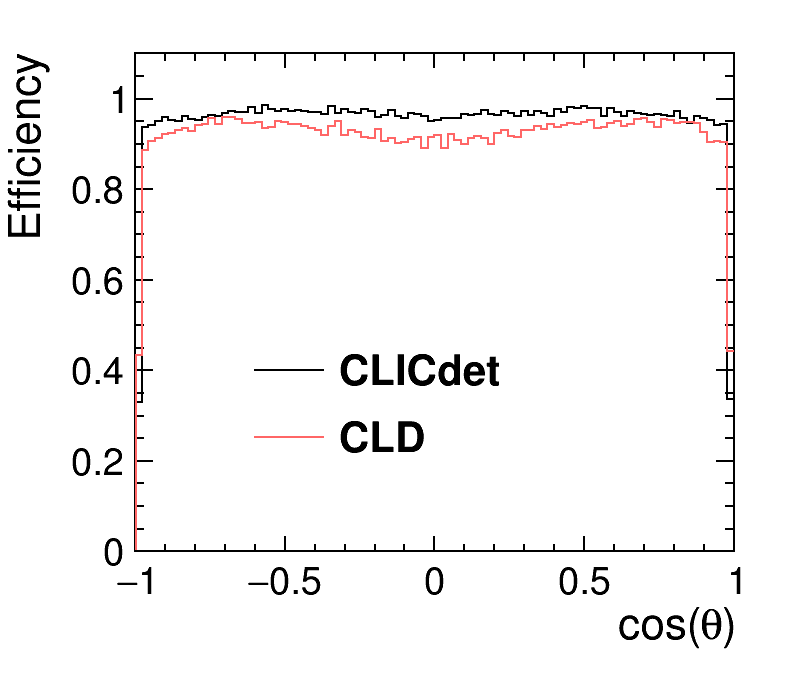
\includegraphics[width=6.2cm]{partEff/experimental_v1/calice_CLIC_vs_FCCee_effVsTheta_pions_E100.pdf}};
    
    \node  at (\xRefPosOne+4.5,\yRefPosOne+3.6) (box){%
    \myCenterBox{\small 100 GeV pions}
    }; 
    \node[inner sep=0pt] (tmp) at (\xRefPosOne-3.9,\yRefPosOne+3.6)
    {\tiny WORK IN PROGRESS};
    \node[inner sep=0pt] (tmp) at (\xRefPosOne+2.1,\yRefPosOne+3.6)
    {\tiny WORK IN PROGRESS};
    
\node  at (\xRefPosOne,\yRefPosOne-2.8) (box){%
\begin{minipage}{\textwidth}
  \begin{itemize}
    \item Type, angular and energy matching with true pion
   \item Pion efficiency is 95-96$\%$ for CLICdet and 93-94 $\%$ for CLD
   \item Difference between CLICdet and CLD models are under investigation
  \end{itemize}
\end{minipage}
};


% % HELPER draw advanced helping grid with axises:
% \draw(-0.5,-4) to[grid with coordinates] (11.5,4);
\end{tikzpicture}
 
\end{frame}
%*****************************************************************************
%*****************************************************************************
\begin{frame}{\large \large Single photon efficiency}

\renewcommand{\yRefPosOne}{-0.5}
\renewcommand{\xRefPosOne}{5.5}
\renewcommand{\xRefIncrementOne}{5.5}
\begin{tikzpicture}[overlay]

 \node[inner sep=0pt] (tmp) at (\xRefPosOne-3,\yRefPosOne+1.2)
    {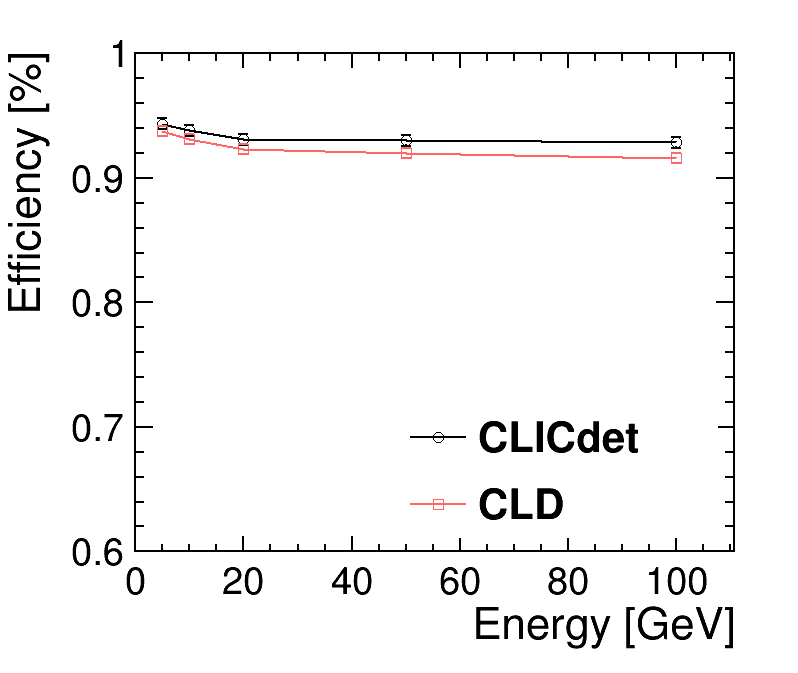
\includegraphics[width=6.2cm]{partEff/experimental_v1/calice_CLIC_vs_FCCee_effVsEnergy_photons.pdf}};
    
 \node[inner sep=0pt] (tmp) at (\xRefPosOne+3,\yRefPosOne+1.25)
    {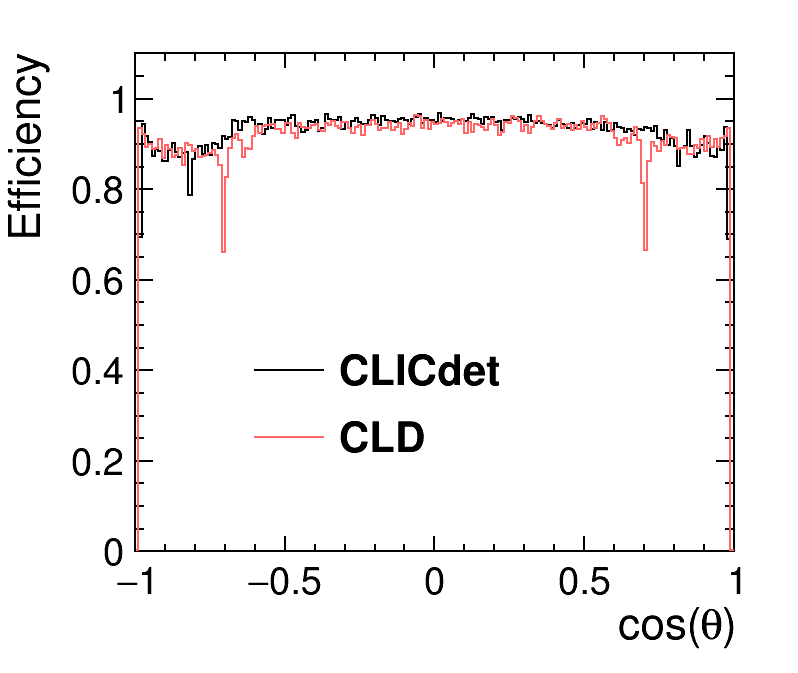
\includegraphics[width=6.2cm]{partEff/experimental_v1/calice_CLIC_vs_FCCee_effVsTheta_photons_E50.pdf}};
    
    \node  at (\xRefPosOne+4.5,\yRefPosOne+3.6) (box){%
    \myCenterBox{\small 50 GeV photons}
    }; 
    \node[inner sep=0pt] (tmp) at (\xRefPosOne-3.9,\yRefPosOne+3.6)
    {\tiny WORK IN PROGRESS};
    \node[inner sep=0pt] (tmp) at (\xRefPosOne+2.1,\yRefPosOne+3.6)
    {\tiny WORK IN PROGRESS};
    
\node  at (\xRefPosOne,\yRefPosOne-2.8) (box){%
\begin{minipage}{\textwidth}
  \begin{itemize}
    \item Type, angular and energy matching with true photon
    \item Photon inefficiency is due to photon conversion which happens late in the tracking system $\to$ two reconstructed photons (likely fails angular and/or energy matching)
%     \item 
  \end{itemize}
\end{minipage}
};


% % HELPER draw advanced helping grid with axises:
% \draw(-0.5,-4) to[grid with coordinates] (11.5,4);
\end{tikzpicture}
 
\end{frame}
%*****************************************************************************
%*****************************************************************************
\begin{frame}{\large \large Single photon efficiency}

\renewcommand{\yRefPosOne}{-0.5}
\renewcommand{\xRefPosOne}{5.5}
\renewcommand{\xRefIncrementOne}{5.5}
\begin{tikzpicture}[overlay]

 \node[inner sep=0pt] (tmp) at (\xRefPosOne-3,\yRefPosOne+1.2)
    {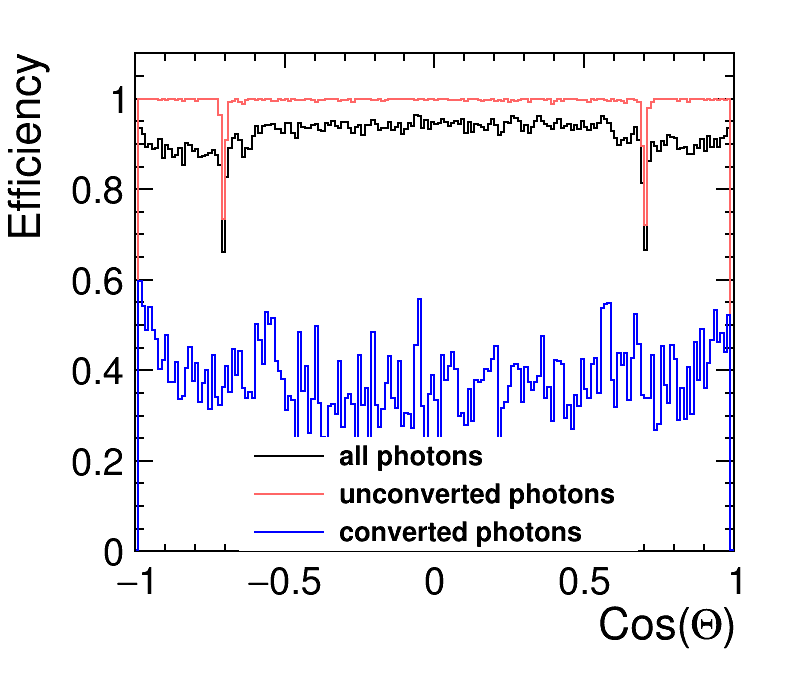
\includegraphics[width=6.2cm]{partEff/experimental_v1/calice_photonConv_plot1.pdf}};
    
 \node[inner sep=0pt] (tmp) at (\xRefPosOne+3,\yRefPosOne+1.25)
    {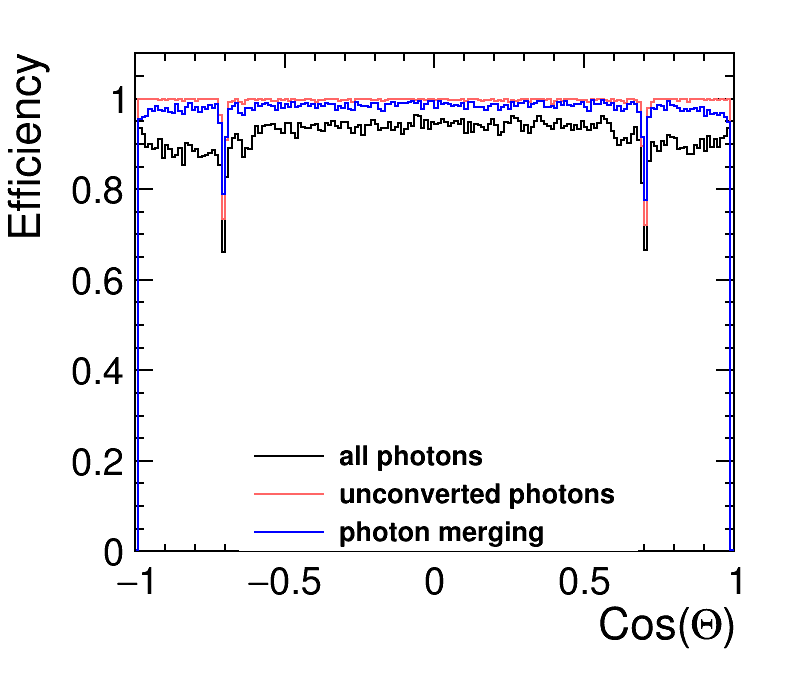
\includegraphics[width=6.2cm]{partEff/experimental_v1/calice_photonConv_plot2.pdf}};
    
            \node  at (\xRefPosOne-1.5,\yRefPosOne+3.6) (box){%
    \myCenterBox{\small CLD}
    }; 
    
    \node  at (\xRefPosOne+4.5,\yRefPosOne+3.6) (box){%
    \myCenterBox{\small 50 GeV photons}
    }; 
    \node[inner sep=0pt] (tmp) at (\xRefPosOne-3.9,\yRefPosOne+3.6)
    {\tiny WORK IN PROGRESS};
    \node[inner sep=0pt] (tmp) at (\xRefPosOne+2.1,\yRefPosOne+3.6)
    {\tiny WORK IN PROGRESS};
    
\node  at (\xRefPosOne,\yRefPosOne-2.8) (box){%
\begin{minipage}{\textwidth}
  \begin{itemize}
    \item Efficiency for unconverted photons reaches 99 $\%$ when efficiency for converted photons is only $\approx$ 30-40 $\%$
    \item merging close photons allows to almost completely recover the efficiency
               
  \end{itemize}
\end{minipage}
};


% % HELPER draw advanced helping grid with axises:
% \draw(-0.5,-4) to[grid with coordinates] (11.5,4);
\end{tikzpicture}
 
\end{frame}
%*****************************************************************************
%*****************************************************************************
\begin{frame}{\large \large Single photon efficiency}

\renewcommand{\yRefPosOne}{-0.5}
\renewcommand{\xRefPosOne}{5.5}
\renewcommand{\xRefIncrementOne}{5.5}
\begin{tikzpicture}[overlay]

 \node[inner sep=0pt] (tmp) at (\xRefPosOne-3,\yRefPosOne+1.2)
    {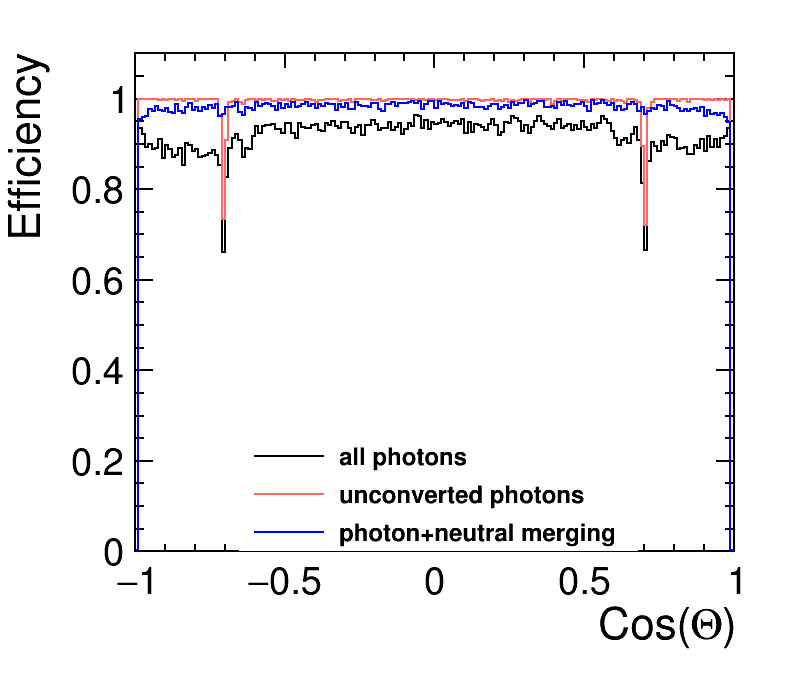
\includegraphics[width=6.2cm]{partEff/experimental_v1/calice_photonConv_plot333.pdf}};
        
 \node[inner sep=0pt] (tmp) at (\xRefPosOne+3,\yRefPosOne+1.25)
    {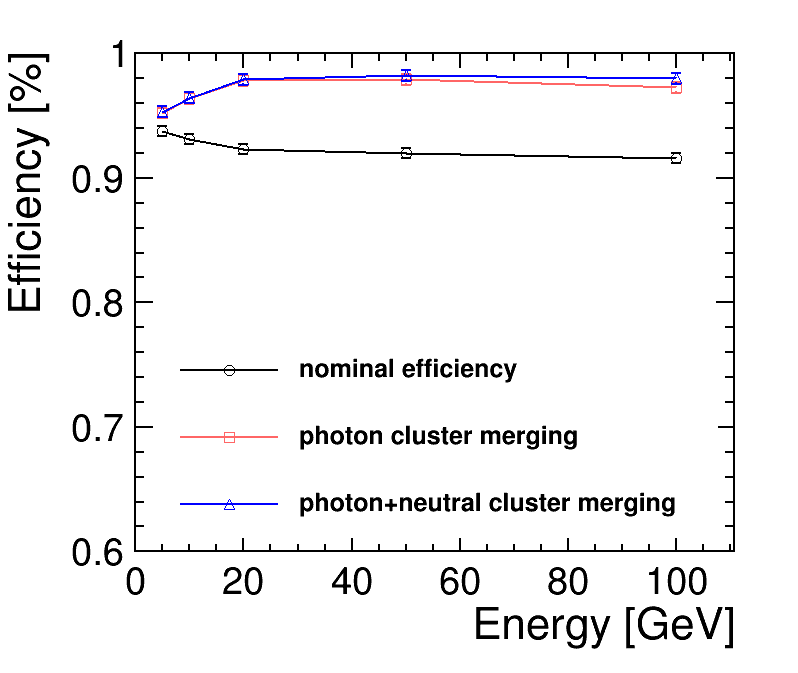
\includegraphics[width=6.2cm]{partEff/experimental_v1/calice_photonEff_vs_energy_reclustering_FCCee.pdf}};
    
            \node  at (\xRefPosOne-1.5,\yRefPosOne+3.6) (box){%
    \myCenterBox{\small CLD}
    }; 
    
    \node  at (\xRefPosOne+4.5,\yRefPosOne+3.6) (box){%
    \myCenterBox{\small 50 GeV photons}
    }; 
    \node[inner sep=0pt] (tmp) at (\xRefPosOne-3.9,\yRefPosOne+3.6)
    {\tiny WORK IN PROGRESS};
    \node[inner sep=0pt] (tmp) at (\xRefPosOne+2.1,\yRefPosOne+3.6)
    {\tiny WORK IN PROGRESS};
    
\node  at (\xRefPosOne,\yRefPosOne-2.8) (box){%
\begin{minipage}{\textwidth}
  \begin{itemize}
    \item Photon calo hits can be split into EM and neutral clusters in calorimeter transition region due to
%     crack in the geometry ({\small space between end of barrel and endcap parts reserved for cables}). 
due to an imperfect overlap between barrel and endcap calorimeters ({\small space between end of barrel and endcap parts reserved for cables})
    \item Merging of close neutral cluster allows recovering efficiency there.
    \item Efficiency reaches 98$\%$ for CLD (similar for CLICdet models)
    
  \end{itemize}
\end{minipage}
};


% % HELPER draw advanced helping grid with axises:
% \draw(-0.5,-4) to[grid with coordinates] (11.5,4);
\end{tikzpicture}
 
\end{frame}
%*****************************************************************************
%*****************************************************************************
\begin{frame}{\large \large Single electron efficiency}

\renewcommand{\yRefPosOne}{-0.5}
\renewcommand{\xRefPosOne}{5.5}
\renewcommand{\xRefIncrementOne}{5.5}
\begin{tikzpicture}[overlay]

 \node[inner sep=0pt] (tmp) at (\xRefPosOne-3,\yRefPosOne+1.2)
    {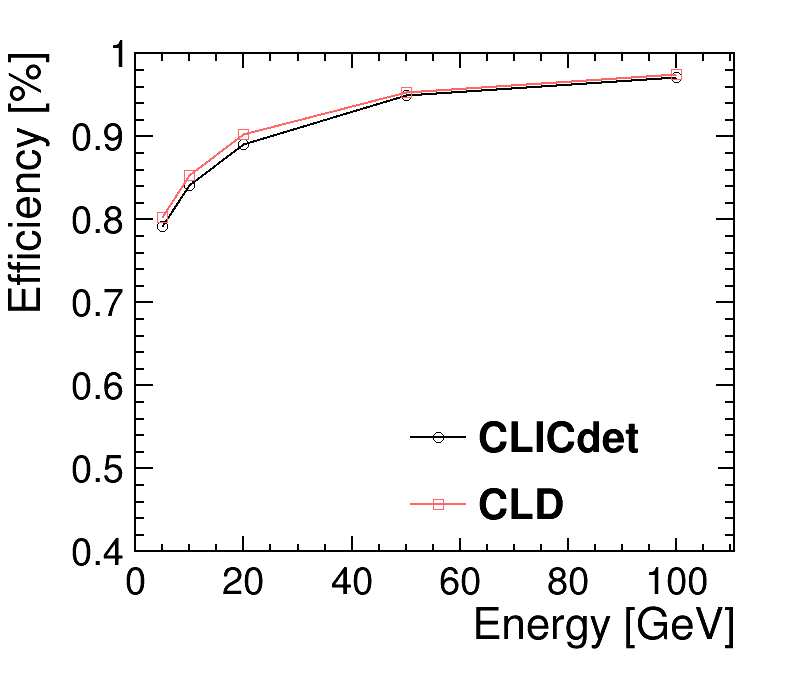
\includegraphics[width=6.2cm]{partEff/experimental_v1/calice_CLIC_vs_FCCee_effVsEnergy_electrons.pdf}};
    
 \node[inner sep=0pt] (tmp) at (\xRefPosOne+3,\yRefPosOne+1.25)
    {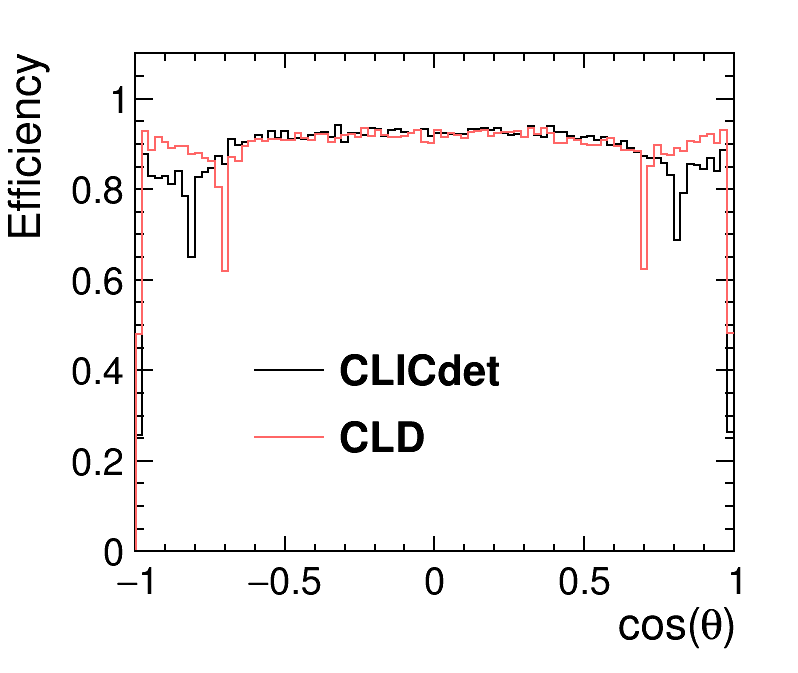
\includegraphics[width=6.2cm]{partEff/experimental_v1/calice_CLIC_vs_FCCee_effVsTheta_electrons_E20.pdf}};
    

    
    \node  at (\xRefPosOne+4.5,\yRefPosOne+3.6) (box){%
    \myCenterBox{\small 20 GeV electrons}
    }; 
    \node[inner sep=0pt] (tmp) at (\xRefPosOne-3.9,\yRefPosOne+3.6)
    {\tiny WORK IN PROGRESS};
    \node[inner sep=0pt] (tmp) at (\xRefPosOne+2.1,\yRefPosOne+3.6)
    {\tiny WORK IN PROGRESS};
    
\node  at (\xRefPosOne,\yRefPosOne-2.8) (box){%
\begin{minipage}{\textwidth}
  \begin{itemize}
    \item study of electron PID efficiency is more complicated due to Bremsstrahlung
    \item impose only particle type matching (no angular and energy matching)
   \item unexpectedly low efficiency for lower energy electrons
  \end{itemize}
\end{minipage}
};


% % HELPER draw advanced helping grid with axises:
% \draw(-0.5,-4) to[grid with coordinates] (11.5,4);
\end{tikzpicture}
 
\end{frame}
%*****************************************************************************
%*****************************************************************************
\begin{frame}{\large \large Single electron efficiency}

\renewcommand{\yRefPosOne}{-0.5}
\renewcommand{\xRefPosOne}{5.5}
\renewcommand{\xRefIncrementOne}{5.5}
\begin{tikzpicture}[overlay]

 \node[inner sep=0pt] (tmp) at (\xRefPosOne-3,\yRefPosOne+1.2)
    {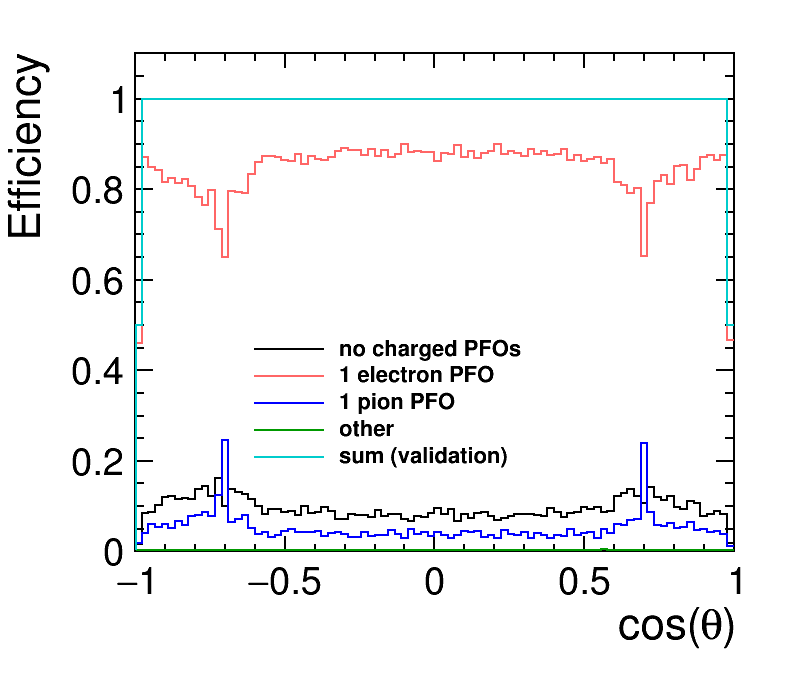
\includegraphics[width=6.2cm]{partEff/experimental_v1/calice_CLIC_vs_FCCee_effVsTheta_fakes_electrons_E10.pdf}};
    
 \node[inner sep=0pt] (tmp) at (\xRefPosOne+3,\yRefPosOne-0.1)
    {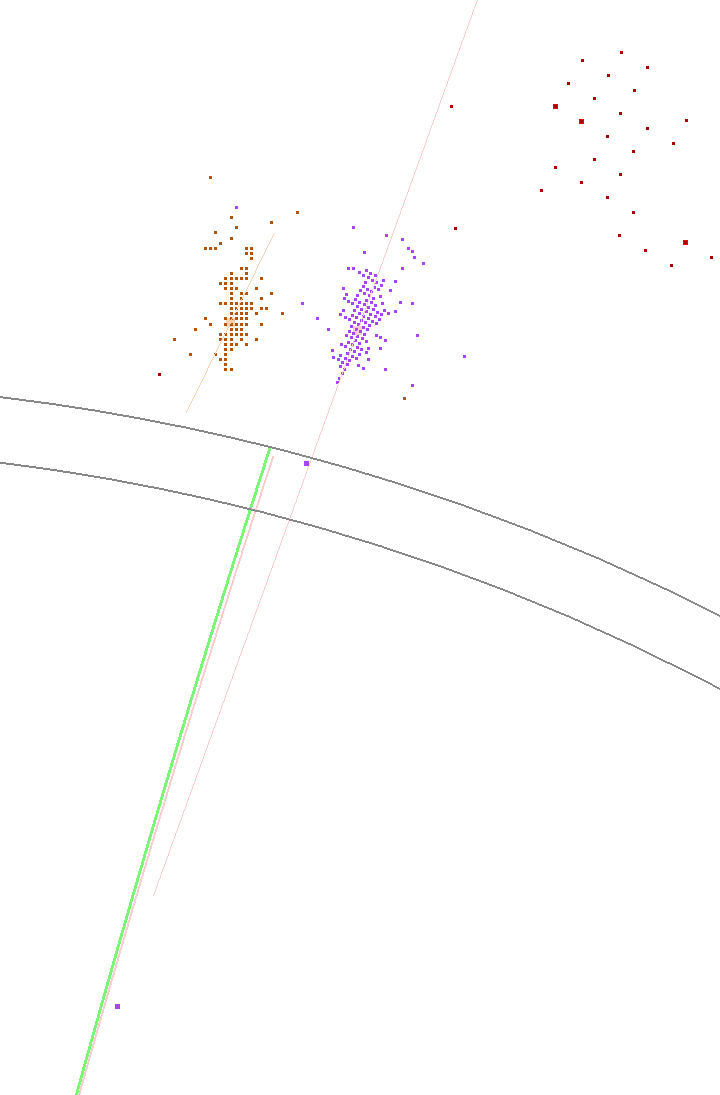
\includegraphics[width=5.5cm]{other/eventDisplay.png}};
    
    \node  at (\xRefPosOne-1.5,\yRefPosOne+3.6) (box){%
    \myCenterBox{\small 10 GeV electrons}
    }; 
    \node[inner sep=0pt] (tmp) at (\xRefPosOne-3.9,\yRefPosOne+3.6)
    {\tiny WORK IN PROGRESS};
%     \node[inner sep=0pt] (tmp) at (\xRefPosOne+2.1,\yRefPosOne+3.6)
%     {\tiny WORK IN PROGRESS};
    
\node  at (\xRefPosOne-3.2,\yRefPosOne-2.8) (box){%
\begin{minipage}{0.6\textwidth}
  \begin{itemize}
    \item in 10-13$\%$ of events no charged PFO is reconstructed in the event
    \item track-cluster association algorithm fails to attach track to cluster (as shown on the right) \\[0.3cm]
    \item in 3-6$\%$ of events fake ``pion'' is reconstructed 
    \item in calorimeter transition region a small fraction of electrons is reconstructed as ``pions''
  \end{itemize}
\end{minipage}
};


% % HELPER draw advanced helping grid with axises:
% \draw(-0.5,-4) to[grid with coordinates] (11.5,4);
\end{tikzpicture}
 
\end{frame}
%*****************************************************************************
%*****************************************************************************
\begin{frame}{\large \large Single electron efficiency: track-cluster association}
 
\renewcommand{\yRefPosOne}{0.4}
\renewcommand{\xRefPosOne}{2.5}
\renewcommand{\xRefIncrementOne}{5.5}
\begin{tikzpicture}[overlay]

 \node[inner sep=0pt] (tmp) at (\xRefPosOne+6,\yRefPosOne-0.1)
    {\includegraphics[width=4.5cm]{other/eventDisplay_zoomed_pict3_v3.pdf}};

\node  at (\xRefPosOne,\yRefPosOne+1) (box){%
  \begin{minipage}{0.6\textwidth}
  Track-cluster association algorithm in Pandora
    \begin{itemize}
    \item Get track state on ECAL inner surface
      \item Loop through all hits within a cluster
      \item Calculate perpendicular and parallel distance between calo hit and track state position with respect to track state direction
      \item Find hit with minimal perpendicular distance $\to$ this value is {\color{red}the track-cluster distance}
      \item Default Pandora settings in electron reconstruction algorithm: the track is matched if track-cluster distance $<$ {\color{red} \bf 10 mm}
      
    \end{itemize}
  \end{minipage}
};

\node at (\xRefPosOne+2.5,\yRefPosOne-3.2) (box){%
  \begin{minipage}{\textwidth}
   Photon reconstruction algorithm
    \begin{itemize}
      \item Second PID algorithm run by Pandora (after muons)
      \item if there is a track within {\color{red} \bf 3 mm} - check if cluster should be discarded since it's probably an electron $\to$ the cluster is likely reconstructed as an electron
      \item otherwise (if track-cluster distance $>$ {\color{red} \bf 3 mm}) consider EM cluster trackless and run photon ID test $\to$ the cluster is likely reconstructed as a photon
    \end{itemize}
  \end{minipage}
};

\node [PixelBox] at (\xRefPosOne+2.9,\yRefPosOne-4.9) (box){%
  \begin{minipage}{\textwidth}
   Vary these 2 parameters to investigate an effect on the electron ID efficiency
  \end{minipage}
};

\end{tikzpicture}

  
\end{frame}
%*****************************************************************************
\begin{frame}{\large \large Single electron efficiency: track-cluster association}
 
\renewcommand{\yRefPosOne}{-4}
\renewcommand{\xRefPosOne}{5.5}
\renewcommand{\xRefIncrementOne}{5.5}
\begin{tikzpicture}[overlay]

 \node[inner sep=0pt] (tmp) at (\xRefPosOne+3,\yRefPosOne+5.5)
    {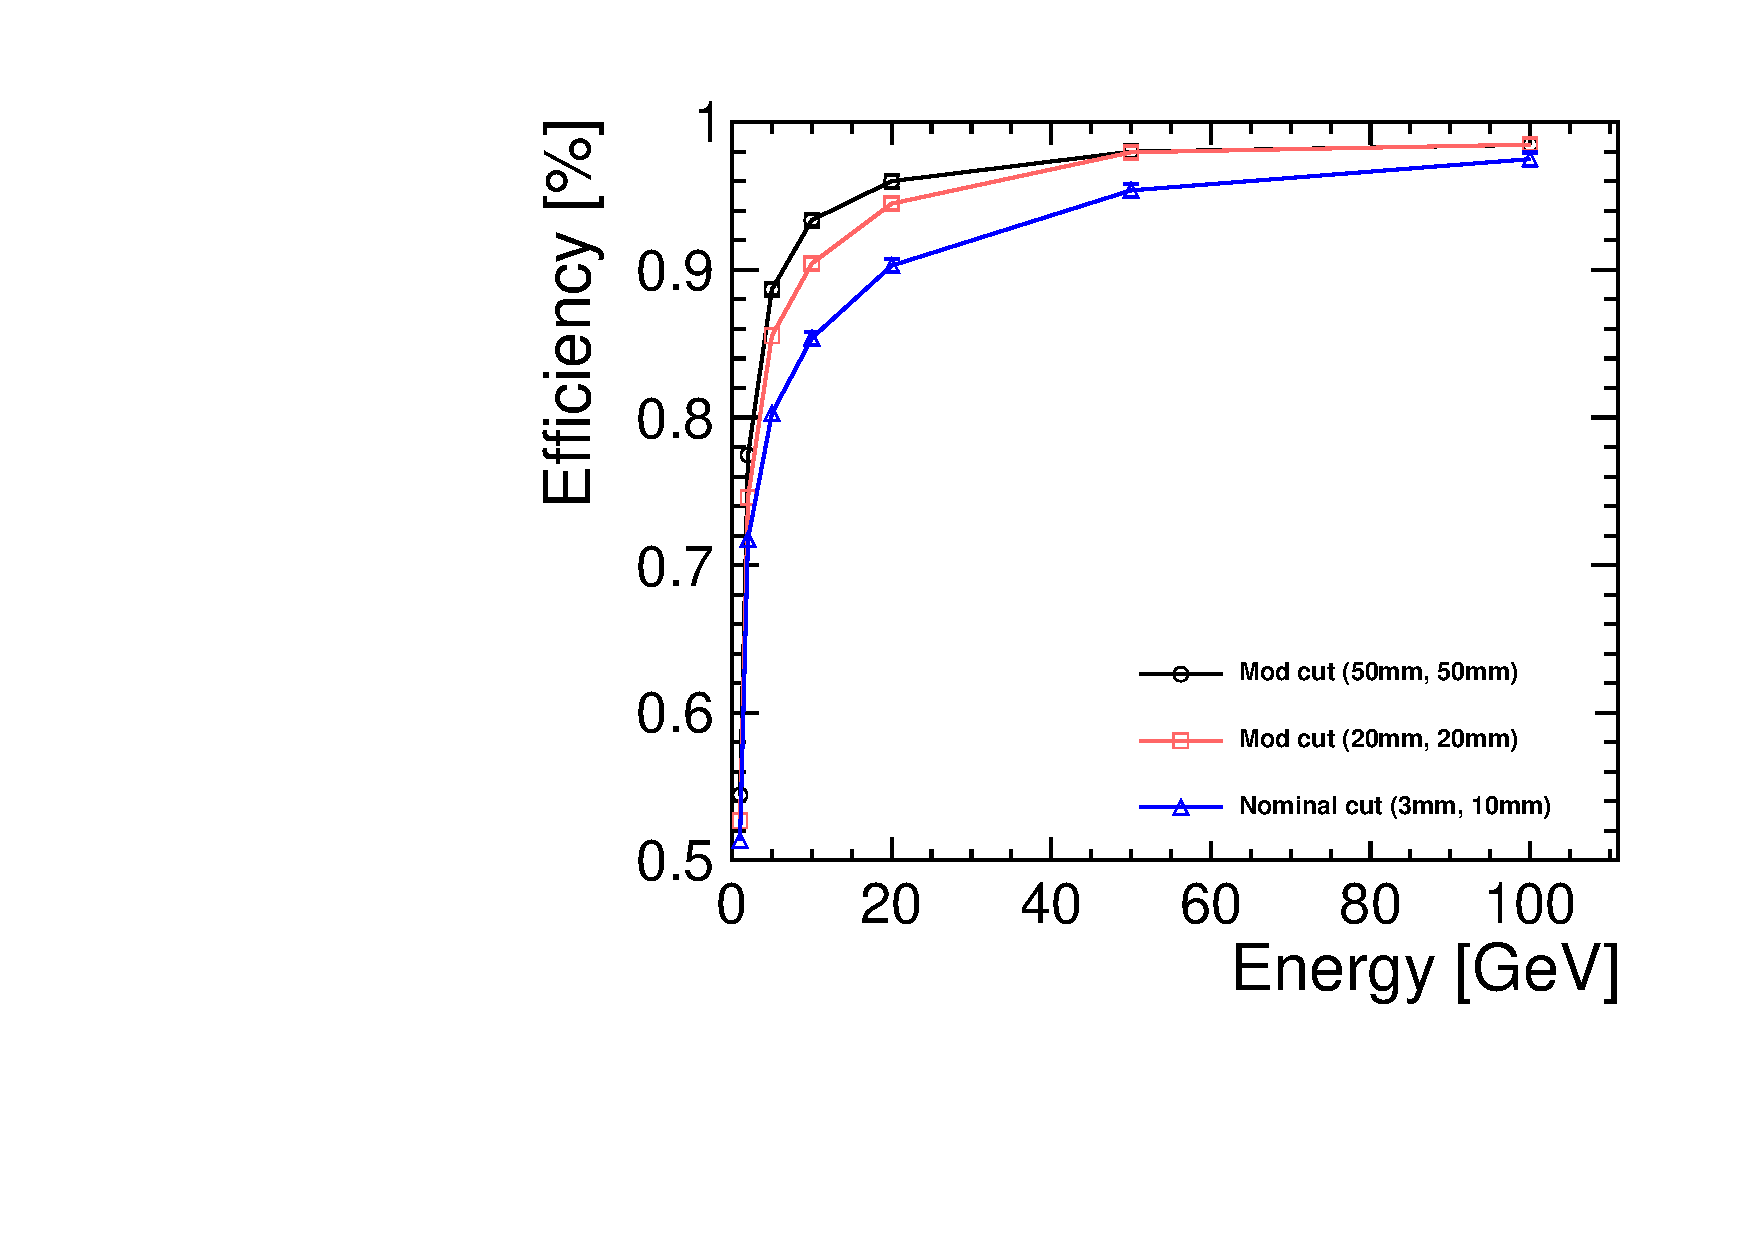
\includegraphics[width=5cm]{partEff/experimental_v1/TrackClusterDistanceCut_effVsEnergy.pdf}};

    \node  at (\xRefPosOne+4,\yRefPosOne+6.2) (box){%
    \myCenterBox{\small Electrons}
    }; 
    \node  at (\xRefPosOne+4,\yRefPosOne+5.8) (box){%
    \myCenterBox{\small CLD}
    }; 
    
 \node[inner sep=0pt] (tmp) at (\xRefPosOne-3,\yRefPosOne+1.2)
    {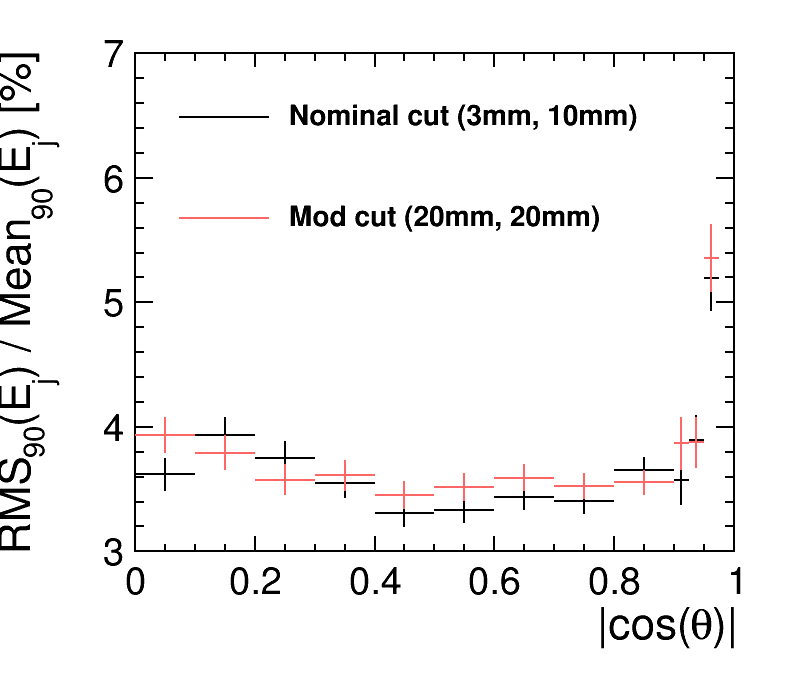
\includegraphics[width=5cm]{partEff/experimental_v1/TrackClusterDistanceCut_resolutionVsCosTheta_Zuds380_nomVs20.pdf}};
    
 \node[inner sep=0pt] (tmp) at (\xRefPosOne+3,\yRefPosOne+1.2)
    {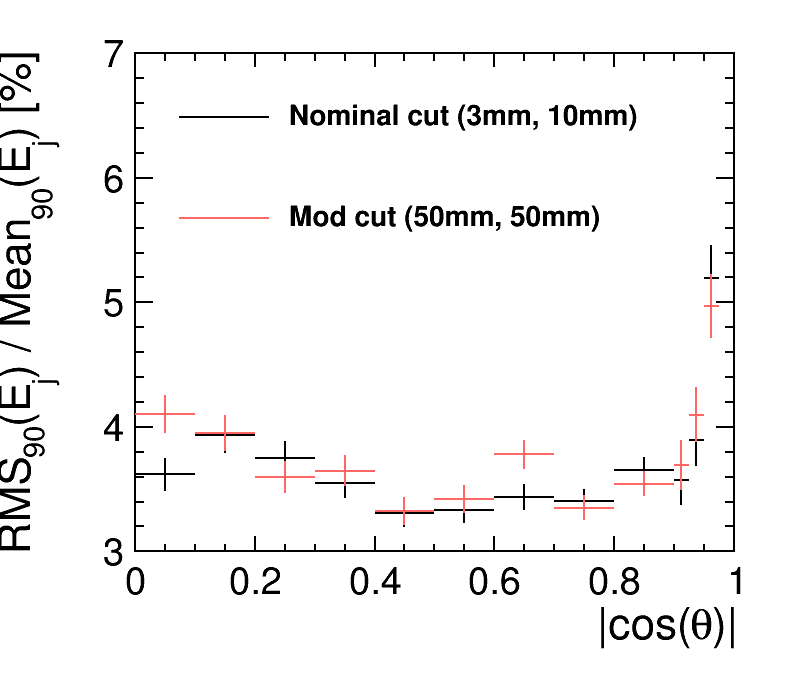
\includegraphics[width=5cm]{partEff/experimental_v1/TrackClusterDistanceCut_resolutionVsCosTheta_Zuds380_nomVs50.pdf}};
     

    \node  at (\xRefPosOne-1.8,\yRefPosOne+3.2) (box){%
    \myCenterBox{\small 190 GeV jets}
    };     
    \node  at (\xRefPosOne+4.2,\yRefPosOne+3.2) (box){%
    \myCenterBox{\small 190 GeV jets}
    }; 
    \node[inner sep=0pt] (tmp) at (\xRefPosOne-3.7,\yRefPosOne+3.2)
    {\tiny WORK IN PROGRESS};
    \node[inner sep=0pt] (tmp) at (\xRefPosOne+2.3,\yRefPosOne+3.2)
    {\tiny WORK IN PROGRESS};
    \node[inner sep=0pt] (tmp) at (\xRefPosOne+2.3,\yRefPosOne+7.5)
    {\tiny WORK IN PROGRESS};
    

\node  at (\xRefPosOne-2.9,\yRefPosOne+5.4) (box){%
  \begin{minipage}{0.6\textwidth}
    \begin{itemize}
      \item compare 3 sets of track-cluster distance cut: \\(3mm, 10mm), (20mm, 20mm), (50mm, 50mm)
      \item Increasing of track-cluster distance requirement allows to recover efficiency 
      \item Improvement of PID efficiency at low energies (85$\% \to$  95$\%$ for 10 GeV electrons)\\[0.5cm]
      \item Loosening track-cluster distance requirement doesn't have a significant impact on jet energy resolution
    \end{itemize}
  \end{minipage}
};

\node at (\xRefPosOne+2.5,\yRefPosOne-4) (box){%
  \begin{minipage}{\textwidth}
    \begin{itemize}
      \item ???
    \end{itemize}
  \end{minipage}
};

\end{tikzpicture}

  
\end{frame}
%*****************************************************************************
%*****************************************************************************
\begin{frame}{}
    \begin{tikzpicture}[overlay]
    \node[right] (textNode) at (3.1,0) {
      {\large \bf ECAL Endcap Geometry}
    };
    \end{tikzpicture}
\end{frame}
%*****************************************************************************
%*****************************************************************************
\begin{frame}{\large \large CLD and CLICdet ECAL Geometry}

\renewcommand{\yRefPosOne}{0}
\renewcommand{\xRefPosOne}{5.3}
\renewcommand{\xRefIncrementOne}{5.5}
\begin{tikzpicture}[overlay]

%  \node[inner sep=0pt] (tmp) at (\xRefPosOne-2.15,\yRefPosOne-0.56)
%     {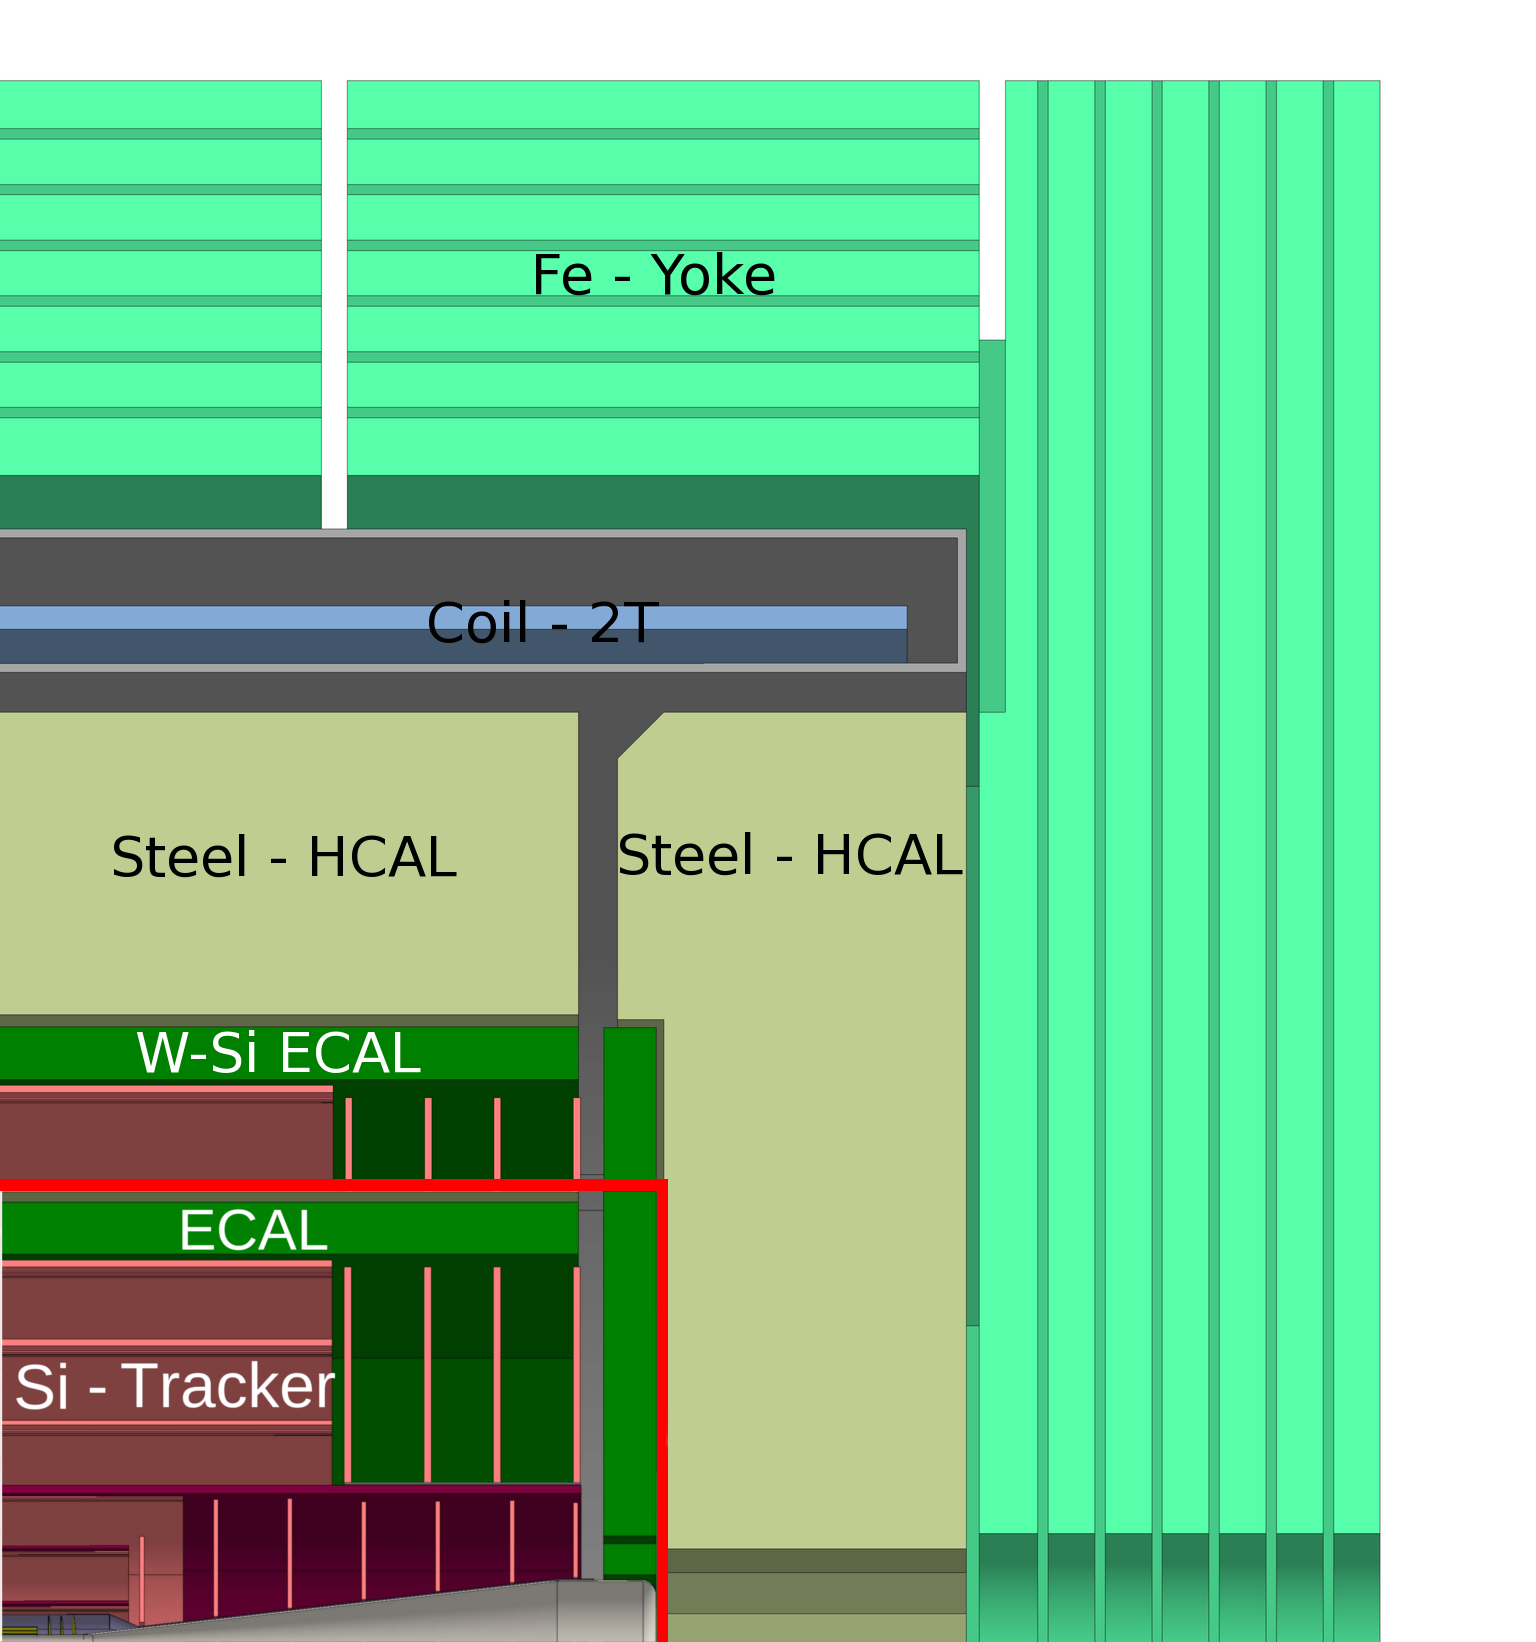
\includegraphics[width=7.8cm]{../CEPC_workshop/FCCeePictsFromKonrad/CLIC_FCC_Top_QuarterView_withLabes_withCLIC.png}};

 \node[inner sep=0pt] (tmp) at (\xRefPosOne,\yRefPosOne-0.56)
    {\includegraphics[width=8.5cm]{/home/oviazlo/Desktop/beamerPresentations/FCCee/pictures/plots_mar14_1018/CLIC_FCC_ECAL.png}};


\node  at (\xRefPosOne+0.6,\yRefPosOne+1.3) (box){%
\myCenterBox{\small CLD model}
}; 

\node  at (\xRefPosOne+0.6,\yRefPosOne-4.2) (box){%
\myCenterBox{\small CLICdet}
}; 
    
%     \draw[black, thick, ->] (-0.8,-4.76)--(-0.8,3.7) node[pos=0.95, right]{\small R [m]};
%     \draw[black, thick, ->] (-0.8,-4.76)--(6.5,-4.76) node[pos=0.95, below]{\tiny Z [m]};
%     
%   \node[inner sep=0pt] (tmp) at (\xRefPosOne-3.05,\yRefPosOne-4.9)
%     {2.3};   
%   \node[inner sep=0pt] (tmp) at (\xRefPosOne-1.14,\yRefPosOne-4.9)
%     {3.7};  

%% HELPER draw advanced helping grid with axises:
% \draw(-0.5,-4) to[grid with coordinates] (11.5,4);
\end{tikzpicture}

 
\end{frame}
%*****************************************************************************
%*****************************************************************************
\begin{frame}{\large \large ECAL material budget}

\renewcommand{\yRefPosOne}{-0.5}
\renewcommand{\xRefPosOne}{5.5}
\renewcommand{\xRefIncrementOne}{5.5}
\begin{tikzpicture}[overlay]

 \node[inner sep=0pt] (tmp) at (\xRefPosOne-3,\yRefPosOne+1.2)
    {\includegraphics[width=6.2cm]{/home/oviazlo/Desktop/beamerPresentations/FCCee/pictures/plots_mar14_1018/materialBudget_fccee_vs_clic.pdf}};
    
 \node[inner sep=0pt] (tmp) at (\xRefPosOne+3,\yRefPosOne+1.25)
    {\includegraphics[width=6.2cm]{/home/oviazlo/Desktop/beamerPresentations/FCCee/pictures/plots_mar14_1018/materialBudget.pdf}};

% \node  at (\xRefPosOne+4.1,\yRefPosOne+2.4) (box){%
% \myCenterBox{\small 50 GeV muons}
% }; 



\node  at (\xRefPosOne,\yRefPosOne-2.8) (box){%
\begin{minipage}{\textwidth}
  \begin{itemize}
   \item crack in ECAL transition region - the main reason for photon inefficiency
   \item extend ECAL endcap in the same way as done in CLIC
   \item extend the outer radius of ECAL endcap: 2350 mm $\to$ 2455 mm
  \end{itemize}
\end{minipage}
};


% % HELPER draw advanced helping grid with axises:
% \draw(-0.5,-4) to[grid with coordinates] (11.5,4);
\end{tikzpicture}
 
\end{frame}
%*****************************************************************************
%*****************************************************************************
\begin{frame}{\large \large Photon and Electron efficiencies}

\renewcommand{\yRefPosOne}{-0.5}
\renewcommand{\xRefPosOne}{5.5}
\renewcommand{\xRefIncrementOne}{5.5}
\begin{tikzpicture}[overlay]

 \node[inner sep=0pt] (tmp) at (\xRefPosOne-3,\yRefPosOne+1.2)
    {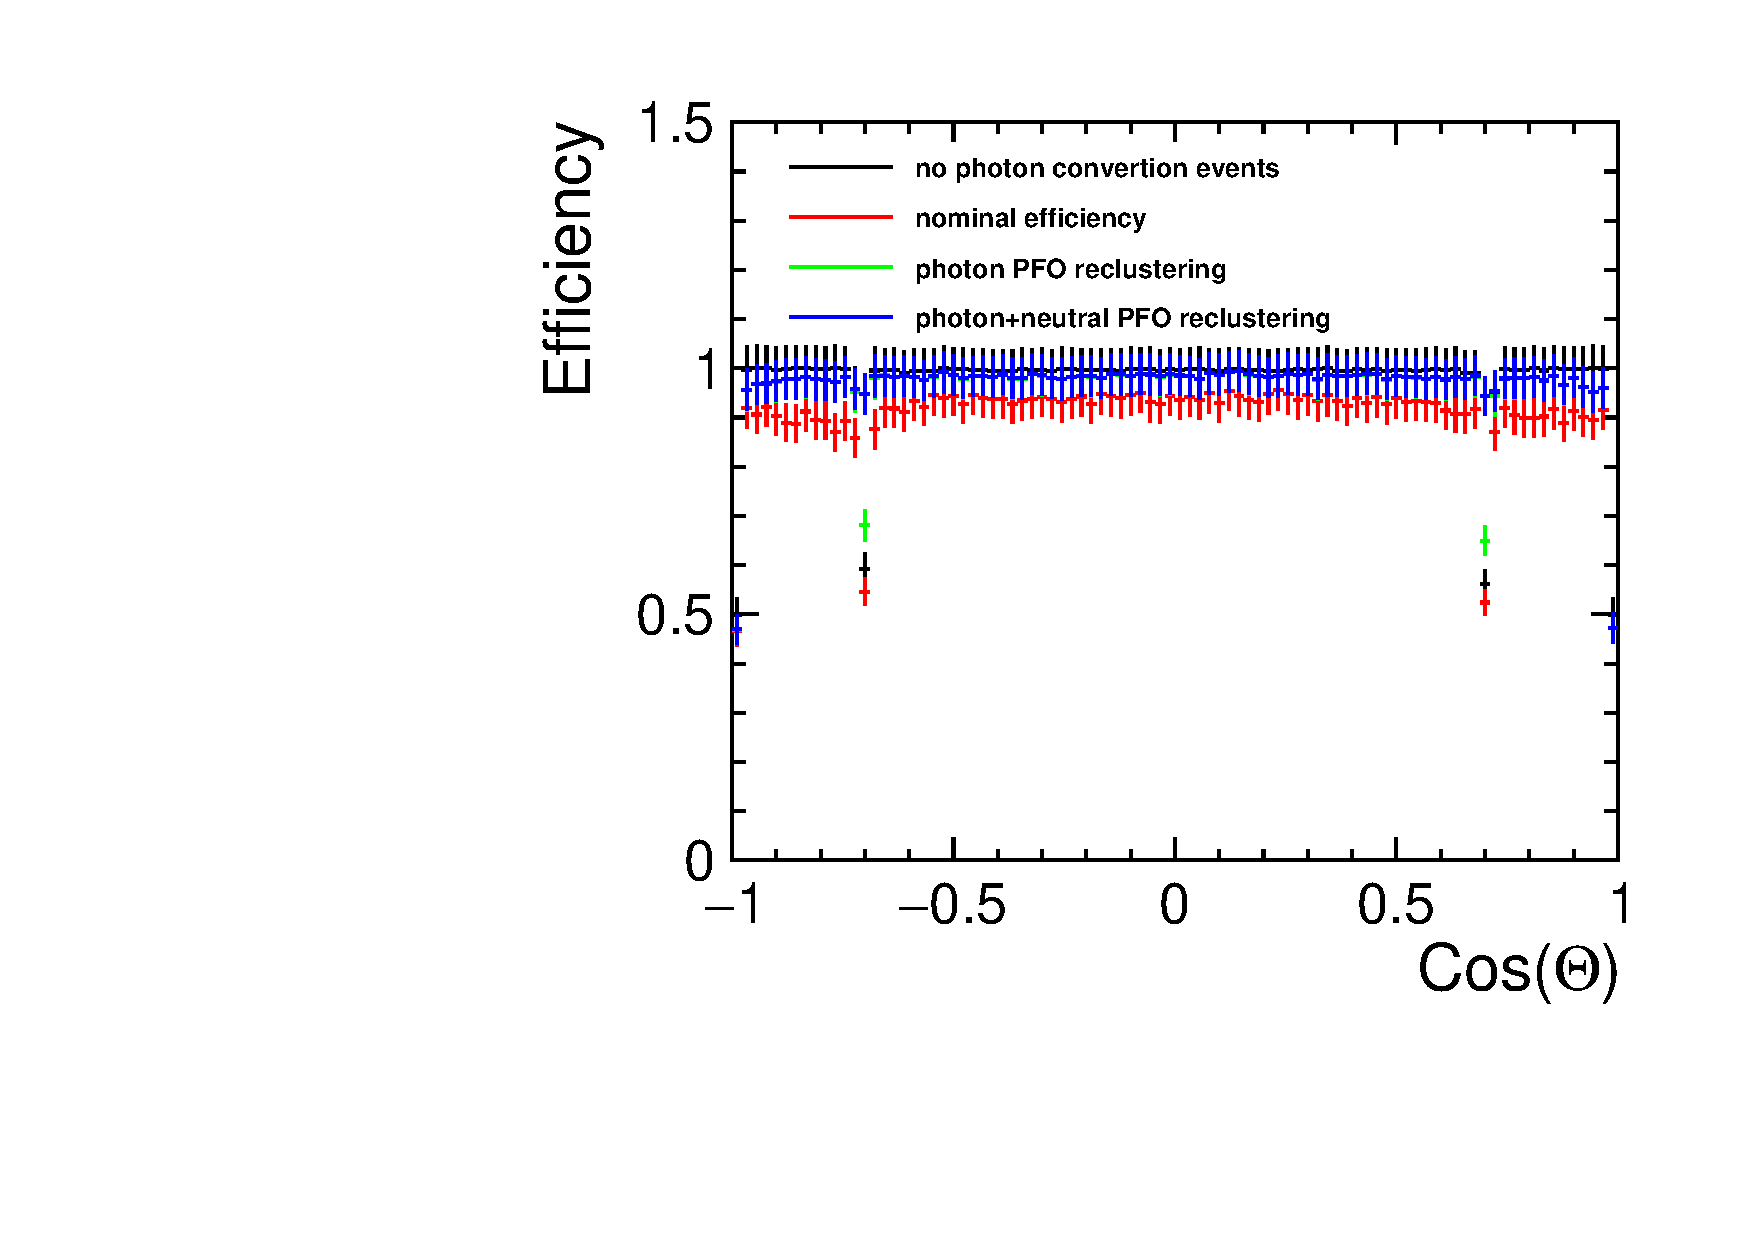
\includegraphics[width=6.2cm]{/home/oviazlo/Desktop/beamerPresentations/FCCee/pictures/plots_mar14_1018/photon_eff_vs_theta_E100.pdf}};
    
 \node[inner sep=0pt] (tmp) at (\xRefPosOne+3,\yRefPosOne+1.25)
    {\includegraphics[width=6.2cm]{/home/oviazlo/Desktop/beamerPresentations/FCCee/pictures/plots_mar14_1018/extendedEcalEndcap_effVsTheta_electrons_E50_fcceeComp.pdf}};

  \node  at (\xRefPosOne-1.5,\yRefPosOne+3.6) (box){%
    \myCenterBox{\small 100 GeV photons}
    }; 
    
  \node  at (\xRefPosOne+4.5,\yRefPosOne+3.6) (box){%
    \myCenterBox{\small 50 GeV electrons}
    }; 



\node  at (\xRefPosOne,\yRefPosOne-2.8) (box){%
\begin{minipage}{\textwidth}
  \begin{itemize}
   \item extension of ECAL endcap recover photon inefficiency in transition region
  \end{itemize}
\end{minipage}
};


% % HELPER draw advanced helping grid with axises:
% \draw(-0.5,-4) to[grid with coordinates] (11.5,4);
\end{tikzpicture}
 
\end{frame}
%*****************************************************************************
%*****************************************************************************
\begin{frame}{}
    \begin{tikzpicture}[overlay]
    \node[right] (textNode) at (3.1,0) {
      {\large \bf Jet Energy Resolution}
    };
    \end{tikzpicture}
\end{frame}
%*****************************************************************************
%*****************************************************************************
\begin{frame}{\large \large Jet Energy Resolution}

\renewcommand{\yRefPosOne}{-0.5}
\renewcommand{\xRefPosOne}{5.5}
\renewcommand{\xRefIncrementOne}{5.5}
\begin{tikzpicture}[overlay]

 \node[inner sep=0pt] (tmp) at (\xRefPosOne-3,\yRefPosOne+1.2)
    {\includegraphics[width=6.2cm]{/home/oviazlo/Desktop/beamerPresentations/FCCee/pictures/plots_mar14_1018/CLICbyMatthias_vs_FCCee_Zuds91.pdf}};
    
 \node[inner sep=0pt] (tmp) at (\xRefPosOne+3,\yRefPosOne+1.25)
    {\includegraphics[width=6.2cm]{/home/oviazlo/Desktop/beamerPresentations/FCCee/pictures/plots_mar14_1018/CLICbyMatthias_vs_FCCee_Zuds380.pdf}};

  \node  at (\xRefPosOne-1.5,\yRefPosOne+3.6) (box){%
    \myCenterBox{\small 45 GeV Jets}
    }; 
    
  \node  at (\xRefPosOne+4.5,\yRefPosOne+3.6) (box){%
    \myCenterBox{\small 190 GeV Jets}
    }; 



\node  at (\xRefPosOne,\yRefPosOne-2.5) (box){%
\begin{minipage}{\textwidth}
Energy ``Regularisation'' Techniques in Pandora:
  \begin{itemize}
   \item \textbf{MaxHCalHitHadronicEnergy} - 
        Truncates high cell energy to certain threshold
    \item \textbf{SoftwareCompensation} - Adjusts neutral hadron energies based on energy density of calorimeter hits and energy of the cluster the hit belongs to.
  \end{itemize}
\end{minipage}
};

\node  at (\xRefPosOne,\yRefPosOne-3.8) (box){%
\begin{minipage}{\textwidth}
  \begin{itemize}
   \item Try SoftwareCompensation with FCCee
  \end{itemize}
\end{minipage}
};


% % HELPER draw advanced helping grid with axises:
% \draw(-0.5,-4) to[grid with coordinates] (11.5,4);
\end{tikzpicture}
 
\end{frame}
%*****************************************************************************
\backupbegin
%*****************************************************************************
\begin{frame}
\frametitle{BACKUP} 
 
\end{frame}
%*****************************************************************************
%*****************************************************************************
\begin{frame}{\large \large Jet Energy Resolution}

\renewcommand{\yRefPosOne}{-0.5}
\renewcommand{\xRefPosOne}{5.5}
\renewcommand{\xRefIncrementOne}{5.5}
\begin{tikzpicture}[overlay]

 \node[inner sep=0pt] (tmp) at (\xRefPosOne-3,\yRefPosOne+1.2)
    {\includegraphics[width=6.2cm]{/home/oviazlo/Desktop/beamerPresentations/FCCee/pictures/plots_mar14_1018/CLICbyMatthias_vs_FCCee_Zuds91.pdf}};
    
 \node[inner sep=0pt] (tmp) at (\xRefPosOne+3,\yRefPosOne+1.25)
    {\includegraphics[width=6.2cm]{/home/oviazlo/Desktop/beamerPresentations/FCCee/pictures/plots_mar14_1018/CLICbyMatthias_vs_FCCee_Zuds91_extendedEcalEndcap.pdf}};

  \node  at (\xRefPosOne-1.5,\yRefPosOne+3.6) (box){%
    \myCenterBox{\small 45 GeV Jets}
    }; 
    
  \node  at (\xRefPosOne+4.5,\yRefPosOne+3.6) (box){%
    \myCenterBox{\small 190 GeV Jets}
    }; 



\node  at (\xRefPosOne,\yRefPosOne-2.8) (box){%
\begin{minipage}{\textwidth}
  \begin{itemize}
   \item transition region: bin 0.6 $< cos(\theta) <$ 0.7
   \item extension of ECAL endcap slightly improves resolution in transition region but still is worse than  CLIC
  \end{itemize}
\end{minipage}
};


% % HELPER draw advanced helping grid with axises:
% \draw(-0.5,-4) to[grid with coordinates] (11.5,4);
\end{tikzpicture}
 
\end{frame}
%*****************************************************************************
\backupend

\end{document}

